\documentclass[../rapport_MVEX01-11-05]{subfiles}
\begin{document}

\subsection{Egenskaper}

\paragraph{Observationer i egenskapsrumet}

Ny figur med endast de statiska gesterna, förklara vilka som ser ut
att fungera bäst för att urskilja gester.

\notes{Ny figur med rätt egenskaper och rätt gester!!}

\begin{figure}[htbp]
  \centering
  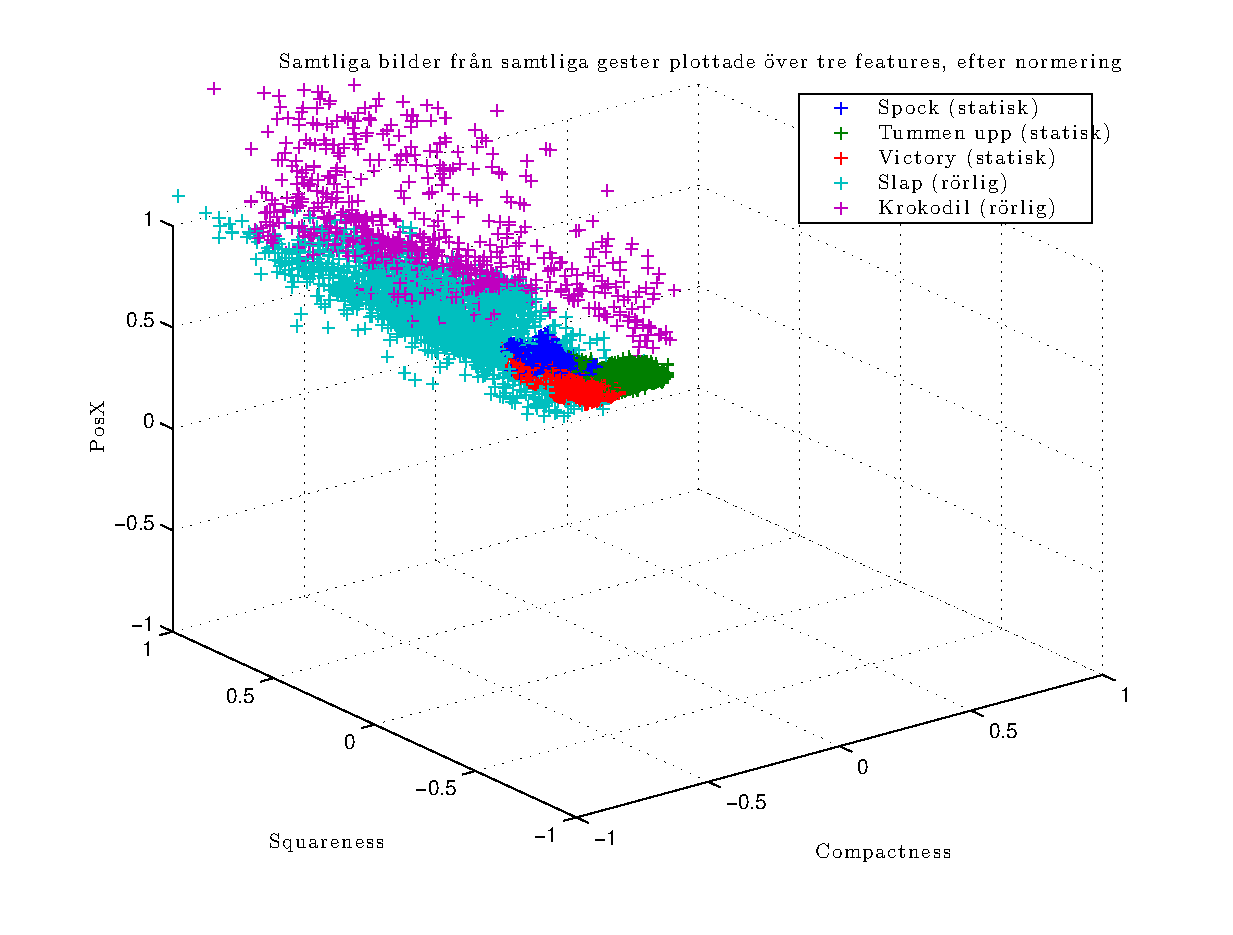
\includegraphics[width=\textwidth]{bilder/feats-1+6+7}
  \caption{De statiska gesterna är betydligt svårare att skilja på än
  de rörliga, vilket illustreras av de tre tydligast grupperande
  egenskaperna.}
  \label{fig:feats167}
\end{figure}

\end{document}